\documentclass[12pt,a4paper]{ctexart}
\usepackage[margin=2.2cm]{geometry}
\usepackage{graphicx,booktabs,amsmath,float,hyperref,xcolor,listings}
\lstset{language=Verilog,basicstyle=\ttfamily\footnotesize,keywordstyle=\color{blue!70!black},commentstyle=\color{green!40!black},stringstyle=\color{orange!60!black},showstringspaces=false,breaklines=true,columns=fullflexible,keepspaces=true,frame=single,tabsize=4}
\setlength{\emergencystretch}{2em}
\newcommand{\reporttitle}{计算机组成与系统结构专题实验\\实验四：存储器阵列设计}
\newcommand{\authname}{李祥熙}
\newcommand{\authid}{2234412799}
\newcommand{\class}{计算机2301}
\title{\reporttitle}
\author{姓名：\authname\quad 班级：\class\\学号：\authid}
\date{2026年11月16日}
\begin{document}
\maketitle
\tableofcontents
\newpage
\section{实验目的}
\begin{itemize}
\item 掌握RAM的地址译码、存储阵列、读写控制、复位和片选功能。
\item 设计1K$\times$16位RAM，用字扩展与位扩展构成4K$\times$32位存储器。
\item 实现选做的双向数据接口，理解写入时外部驱动、读出时存储器驱动的总线约束。
\item 使用初始化文件实现64字指令存储器，按地址异步读取指令。
\item 自主实现32个32位寄存器组成的寄存器文件，支持两个独立读端口、一个写端口及0号寄存器恒零。
\item 编写自检查测试平台，验证全部存储地址和寄存器端口的功能与时序。
\end{itemize}

\section{实验过程}
\subsection{实验环境与时序约定}
实验使用Windows、AMD Vivado 2026.1及其XSim仿真器，采用Verilog语言，工程目标器件为\texttt{xc7a35tcsg324-1}。仿真时间单位为1 ns，精度为1 ps，时钟周期为10 ns。

讲义的RAM示例给出异步描述并注释了同步过程。本实现明确采用时钟上升沿写入、组合逻辑异步读出；复位为高电平有效的异步清零。复位不受片选控制，扩展存储器的所有芯片在复位时一起清零。该阵列描述用于RTL行为验证，整阵列异步清零不作为FPGA块RAM推断的要求。

指令存储器不设置时钟和写端口，仿真开始时装入内容，之后随地址变化输出数据。寄存器文件使用同步写入和两个异步读端口，另外提供异步复位以便建立确定的测试状态。

\subsection{实现与验证步骤}
首先编写1K$\times$16基础芯片，再实例化八片组成4K$\times$32阵列。双向接口封装复用基础芯片，在同一条数据线上交替进行读写。随后完成指令ROM和32$\times$32寄存器文件。

测试平台主要在下降沿安排写入地址和数据，在上升沿之后等待1 ns检查写入结果；异步读取改变地址后等待1 ns检查。先用少量定向操作产生便于阅读的波形，再遍历全部地址或执行固定种子的随机激励。比较使用四态不等运算符，异常未知态或高阻态会导致检查失败。所有断言通过后才打印通过信息。

\section{实验内容}
\subsection{1K$\times$16位双数据线RAM}
存储阵列含1024个16位字，需要10位字地址。输入数据\texttt{din}和输出数据\texttt{dout}分开，控制端\texttt{cs}、\texttt{re}、\texttt{we}均为高有效。
\begin{table}[H]
\centering
\caption{基础RAM读写控制约定}
\begin{tabular}{ccccl}
\toprule
复位 & CS & RE & WE & 行为\\
\midrule
1 & 任意 & 任意 & 任意 & 全阵列清零，输出高阻\\
0 & 0 & 任意 & 任意 & 不写入，输出高阻\\
0 & 1 & 1 & 0 & 异步读出指定字\\
0 & 1 & 0 & 1 & 上升沿写入，输出高阻\\
0 & 1 & 0 & 0 & 保持阵列，输出高阻\\
0 & 1 & 1 & 1 & 不写入，输出高阻\\
\bottomrule
\end{tabular}
\end{table}
读写同时有效时采用确定的无操作策略，避免控制冲突。写入过程只在片选有效且读使能无效时执行，读输出则通过连续赋值控制：
\begin{lstlisting}
else if(cs && we && !re) mem[addr] <= din;
assign dout = (cs && re && !we && !rst) ? mem[addr] : 16'bz;
\end{lstlisting}
第一行位于时钟触发过程内，只有上升沿会改变存储内容；第二行异步响应地址和控制变化。输出高阻表示释放线路，不会把0主动送入其他芯片共享的数据线。

\subsection{4K$\times$32位存储器的字扩展与位扩展}
目标容量为4096个32位字，使用12位字地址。每两片1K$\times$16芯片并联构成一组1K$\times$32：低片连接数据低16位，高片连接高16位。四组再通过高位地址译码实现字扩展，总共需要：
\begin{equation}
\frac{4096}{1024}\times\frac{32}{16}=4\times2=8\text{片}.
\end{equation}
容量由基础芯片的2 KiB扩展为总计16 KiB。地址高两位$A[11:10]$选择组号，低10位$A[9:0]$作为组内地址，各组的地址范围为：
\begin{table}[H]
\centering
\caption{4K存储器的地址分组}
\begin{tabular}{cccc}
\toprule
组号 & 高两位 & 字地址范围（十六进制） & 片选向量\\
\midrule
0 & 00 & 000--3FF & 0001\\
1 & 01 & 400--7FF & 0010\\
2 & 10 & 800--BFF & 0100\\
3 & 11 & C00--FFF & 1000\\
\bottomrule
\end{tabular}
\end{table}
片选还与外部\texttt{cs}相与。读出时，选中组的两片芯片分别驱动高低半字，未选中组输出高阻。写入时，各片共用时钟、组内地址和读写控制，只有选中组存入数据。全地址读回检查可发现组间地址混叠、数据高低半字接错等问题。

\subsection{双向数据线存储器}
选做部分使用\texttt{inout}接口，将输入输出合并为一条数据线。控制\texttt{wr=1}表示读，\texttt{wr=0}表示写，与讲义基础封装的读写极性一致。1K$\times$16双向芯片内部复用双数据线RAM，输入接数据总线，输出也接数据总线，再用相同的字扩展、位扩展形成4K$\times$32双向阵列。

测试平台作为外部总线主机，通过\texttt{drive}决定是否驱动数据。写入时主机驱动\texttt{din}，芯片输出高阻；读出前主机将总线置为高阻，片选芯片才驱动读数据。外部驱动方式如下：
\begin{lstlisting}
assign data = drive ? din : 32'bz;
\end{lstlisting}
这里的高阻赋值确保读周期不与芯片争用数据线。片选无效且主机也释放时，总线整体为高阻；片选无效但主机仍驱动时，总线会反映主机数据，而芯片不接收写入。

\subsection{64$\times$32位指令存储器}
指令存储器采用64个32位字、6位字索引地址，使用\texttt{\$readmemh}装入初始化文件，再用连续赋值实现异步输出。地址是字索引，不是字节地址，因此本模块不额外进行除4或低位截取。

初始化文件包含64个十六进制字。前八字作为可识别的指令样例，依次为20010005、20020003、00221820、00222022、00222824、00223025、AC030000和8C070000，其余56字为0。这里验证指令数据的保存和读取，不执行指令。运行脚本把初始化文件复制到仿真工作目录，Vivado工程将其注册为存储器初始化文件，避免依赖讲义示例中的固定磁盘路径。

\subsection{32$\times$32位寄存器文件}
寄存器文件包含32个32位存储单元，写地址和两个读地址各为5位。\texttt{we3}有效且写地址非0时，在时钟上升沿装入\texttt{wd3}；两个读端口根据各自地址独立组合输出。0号寄存器的读取直接返回常数0，同时禁止对其写入。
\begin{lstlisting}
else if(we3 && wa3 != 0) rf[wa3] <= wd3;
assign rd1 = (ra1 == 0) ? 32'b0 : rf[ra1];
assign rd2 = (ra2 == 0) ? 32'b0 : rf[ra2];
\end{lstlisting}
两条读通路可同时选择不同寄存器，不需要互相等待。读写同一非零地址时，上升沿之前读到旧值，非阻塞写入完成后读到新值；本实现不设置时钟沿前的数据旁路。复位优先于写使能，将所有寄存器清零。

\section{实验结果}
\subsection{基础RAM的同步写入与异步读出}
\begin{figure}[H]
\centering
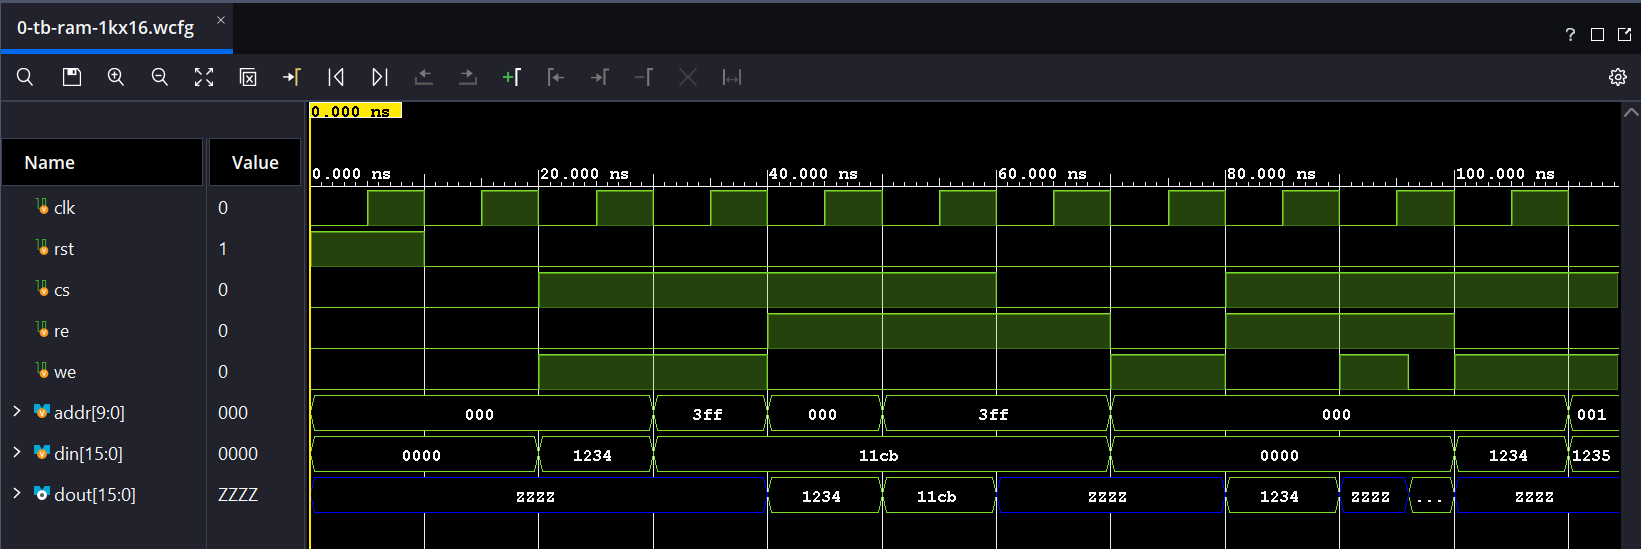
\includegraphics[width=\textwidth]{images/0-tb-ram-1kx16.png}
\caption{基础RAM的同步写入与异步读出}
\end{figure}
测试先写地址000和3FF，数据分别为1234和11CB。写周期输出为高阻，转入读模式后在40 ns、50 ns附近读出对应数据，地址切换不需要等待下一次上升沿。关闭片选后输出恢复高阻。随后在片选无效时尝试写0，再读地址000仍为1234，说明未选中芯片不会改变内容。测试后续还检查读写同时有效时释放输出且不写入。

\subsection{4K$\times$32位存储器的高低半字与片选}
\begin{figure}[H]
\centering
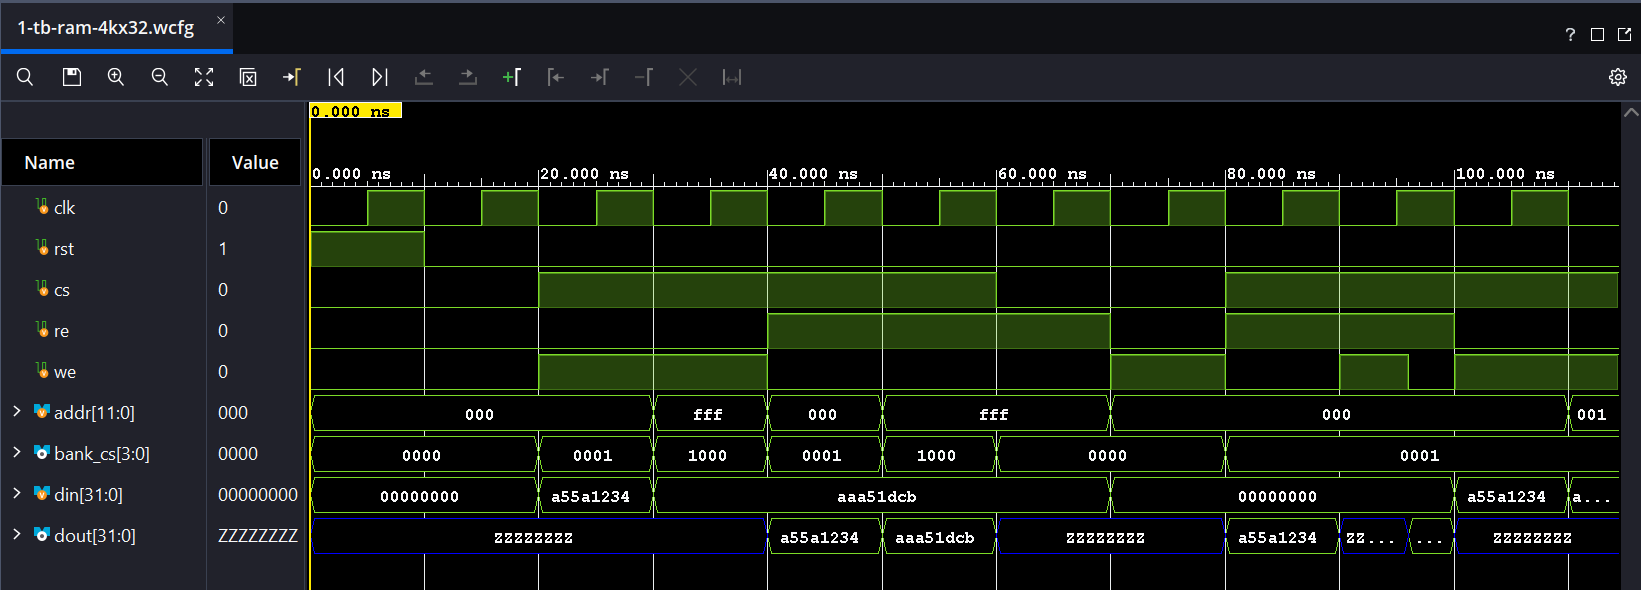
\includegraphics[width=\textwidth]{images/1-tb-ram-4kx32.png}
\caption{4K$\times$32位存储器的高低半字与片选}
\end{figure}
地址000选中第0组，地址FFF选中第3组，片选分别为0001和1000。读出的32位数据分别为A55A1234和AAA51DCB，说明高低16位分别保存并正确汇合，且高位地址能够选择不同组。片选无效时，所有组释放共享输出。

\subsection{跨越3FF与400的组切换}
\begin{figure}[H]
\centering
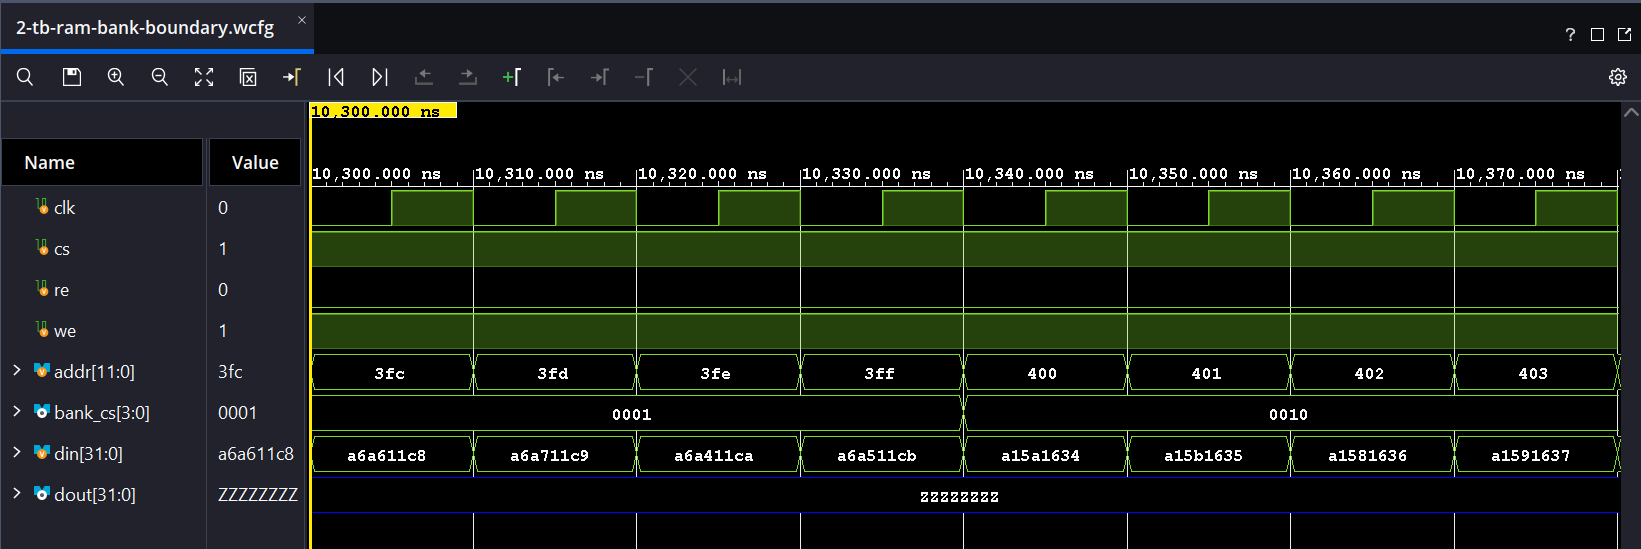
\includegraphics[width=\textwidth]{images/2-tb-ram-bank-boundary.png}
\caption{跨越3FF与400的组切换}
\end{figure}
波形截取连续地址写入过程。地址由3FC、3FD、3FE、3FF进入400后，片选从0001变为0010，低10位组内地址从3FF回到000。输入数据随完整地址变化，写模式下输出保持高阻。随后逐地址读回全部4096个字，验证边界两侧数据没有相互覆盖。

\subsection{双向总线的写驱动与读释放}
\begin{figure}[H]
\centering
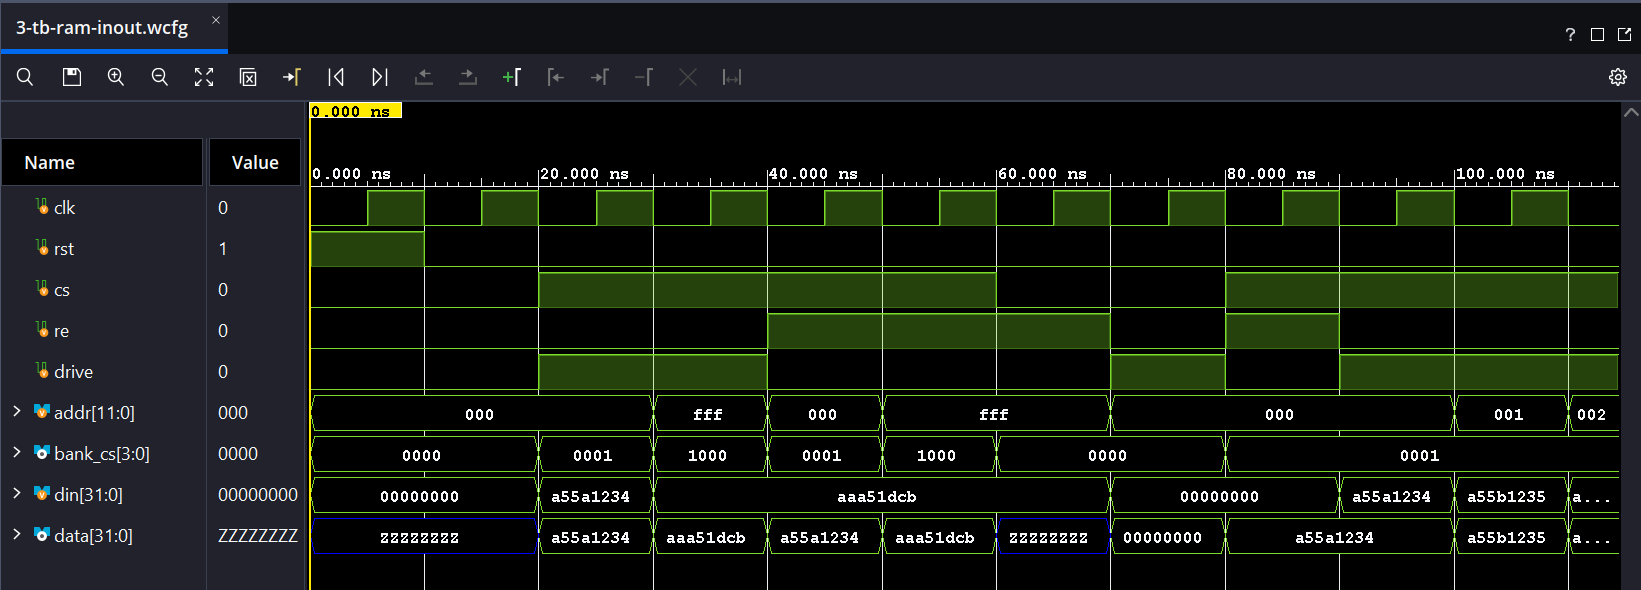
\includegraphics[width=\textwidth]{images/3-tb-ram-inout.png}
\caption{双向总线的写驱动与读释放}
\end{figure}
写周期中drive为1，外部主机把数据送到总线，存储器在上升沿采样。读周期中drive变为0，主机释放线路，由选中存储组输出已保存的数据。片选无效且主机释放时总线为Z。该版本对全部4096个地址执行写入和读回，并在全阵列复位后逐字验证为0。

\subsection{指令ROM的地址与输出对应关系}
\begin{figure}[H]
\centering
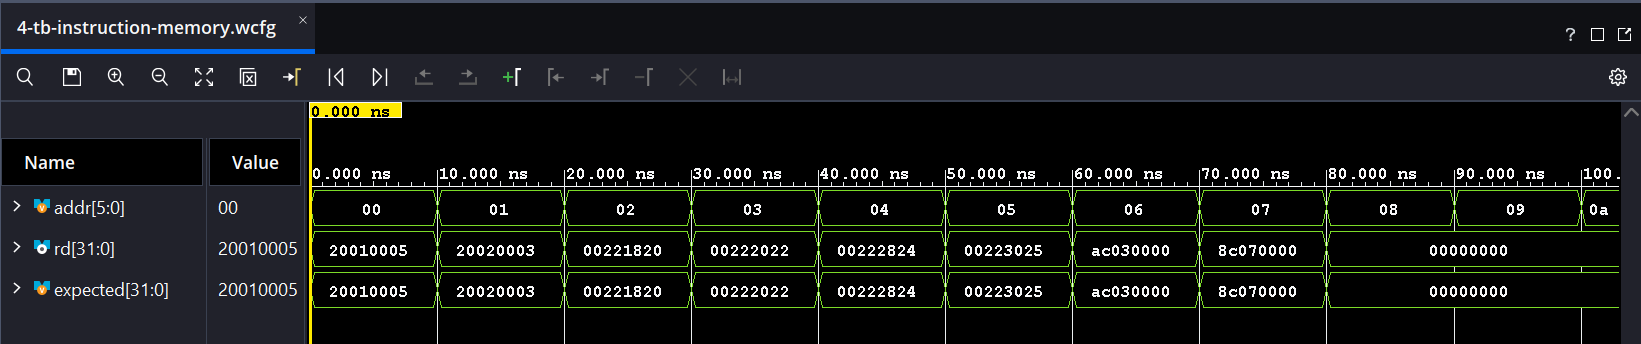
\includegraphics[width=\textwidth]{images/4-tb-instruction-memory.png}
\caption{指令ROM的地址与输出对应关系}
\end{figure}
地址从00递增，输出依次呈现八个初始化指令字，从地址08开始输出0。rd与测试平台中的expected一致。每个地址保持10 ns，读出是组合响应；检查遍历全部64个字，确认初始化文件被正确读取，未装入部分也由文件中的显式零填充。

\subsection{寄存器文件的写入、双端口读出与零寄存器保护}
\begin{figure}[H]
\centering
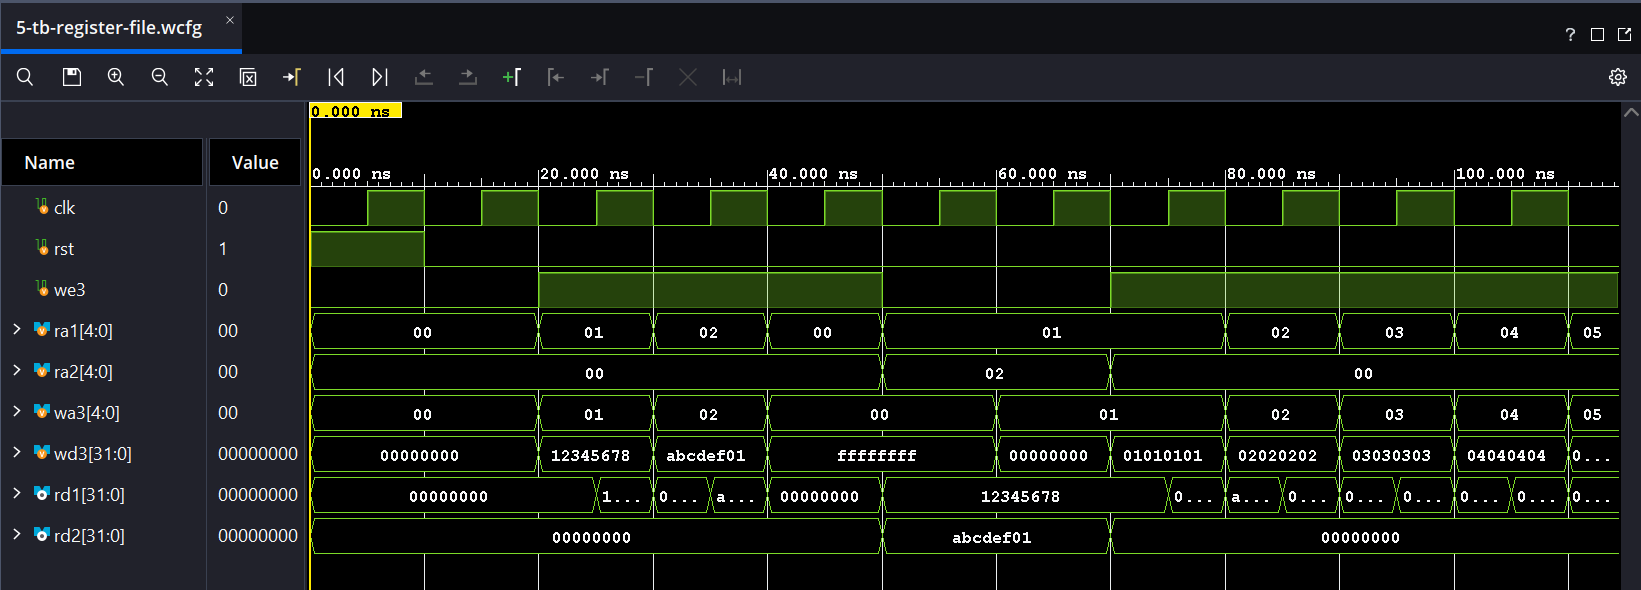
\includegraphics[width=\textwidth]{images/5-tb-register-file.png}
\caption{寄存器文件的写入、双端口读出与零寄存器保护}
\end{figure}
25 ns上升沿向1号寄存器写入12345678，35 ns向2号写入ABCDEF01；45 ns尝试向0号写FFFFFFFF，但两个读取0号的输出仍为0。50 ns附近分别选中1号与2号，两个读端口同时输出各自数据。关闭写使能后，即使写地址和输入数据改变，1号寄存器仍保留原值。随后按顺序写入其余寄存器，并执行随机读写验证。

\subsection{全地址和随机检查结果}
RAM参考数据由地址计算，32位模式为\texttt{A55A1234 XOR (addr * 00010001)}，基础16位芯片取其低16位。地址参与高低半字的数据生成，因此能检查组间覆盖和位宽连接错误。每个RAM测试完成全部地址写入、逐字读回、复位后逐字读零，并补充片选控制检查。

寄存器文件测试用独立参考数组保存期望状态。每次随机周期先在下降沿改变读地址、写地址、写使能及数据，检查沿前读值，再在上升沿更新参考状态并检查沿后输出。固定种子产生1000个周期，最后复位并用两个端口遍历全部32个寄存器。实际运行摘要如下：
\begin{lstlisting}[language={}]
Vivado XSim 2026.1 - Lab 4 self-checking behavioral simulations
Clock period 10 ns; synchronous writes and asynchronous reads.
PASS tb_instruction_memory: all 64 initialized instruction words
PASS tb_ram_1kx16: 1024 address writes/readback, full reset sweep, select and bus controls
PASS tb_ram_4kx32: 4096 address writes/readback, full reset sweep, select and bus controls
PASS tb_ram_inout: 4096 address writes/readback, full reset sweep, select and bus controls
PASS tb_register_file: all 32 registers, zero protection, two read ports, 1000 random cycles, reset
ALL 5 TESTBENCHES PASSED
\end{lstlisting}
五个测试平台均完成编译、展开和仿真。通过信息分别对应64字ROM、1024字基础RAM、两种4096字扩展RAM，以及32个寄存器的读写检查。高阻输出也使用四态比较验证，没有把Z当作普通数值0处理。

\section{总结}
本实验完成基础RAM、八芯片扩展RAM、双向数据接口、指令ROM和32$\times$32寄存器文件，五个自检查测试平台全部通过。六张波形分别展示读写时序、地址分组、跨组边界、总线方向、指令读取和多端口寄存器访问。

字扩展通过高位地址选择存储组，位扩展则由并联芯片分别承担高低数据位，两种扩展共同确定芯片数量与地址分配。高阻控制使未选中的芯片释放共享线路；双向接口还需要外部主机在读周期释放总线。寄存器文件用独立读地址实现并发读取，同时通过读端口常零和写端口屏蔽共同保证0号寄存器的特殊行为。

验证中既检查容易观察的定向波形，也覆盖全部存储地址。同步写入的上升沿前后检查区分了输入数据和已保存状态，异步读检查则验证改变地址后不依赖时钟。完整的初始化文件和固定随机种子使仿真可重复运行。

\clearpage
\section*{附录：完整源代码与运行方法}
\addcontentsline{toc}{section}{附录：完整源代码与运行方法}
以下直接嵌入实际使用的设计文件、测试平台和初始化数据，便于结合正文检查接口与操作时序。
\subsection*{设计模块}
\subsubsection*{\texttt{instruction\_memory.v}}
\begin{lstlisting}
`timescale 1ns / 1ps
module instruction_memory #(parameter INIT_FILE="imem.hex")(
 input wire [5:0] addr,output wire [31:0] rd);
 reg [31:0] mem[0:63];
 initial $readmemh(INIT_FILE,mem);
 assign rd=mem[addr];
endmodule
\end{lstlisting}
初始化文件在仿真开始时加载，6位地址直接索引64字指令阵列。

\subsubsection*{\texttt{ram\_1kx16.v}}
\begin{lstlisting}
`timescale 1ns / 1ps
// Synchronous write, asynchronous read and active-high asynchronous clear.
module ram_1kx16(input wire clk,rst,cs,re,we,input wire [9:0] addr,
 input wire [15:0] din,output wire [15:0] dout);
 reg [15:0] mem[0:1023];integer i;
 always @(posedge clk or posedge rst)
  if(rst) begin for(i=0;i<1024;i=i+1) mem[i]<=0;end
  else if(cs&&we&&!re) mem[addr]<=din;
 assign dout=(cs&&re&&!we&&!rst)?mem[addr]:16'bz;
endmodule
\end{lstlisting}
该基础芯片只在有效写周期的上升沿修改阵列，异步读出和高阻输出由连续赋值决定。复位清零全部1024字。

\subsubsection*{\texttt{ram\_4kx32.v}}
\begin{lstlisting}
`timescale 1ns / 1ps
module ram_4kx32(input wire clk,rst,cs,re,we,input wire [11:0] addr,
 input wire [31:0] din,output wire [31:0] dout);
 wire [3:0] bank_cs;
 genvar b;
 generate for(b=0;b<4;b=b+1)begin:bank
  assign bank_cs[b]=cs&&(addr[11:10]==b);
  ram_1kx16 lo(clk,rst,bank_cs[b],re,we,addr[9:0],din[15:0],dout[15:0]);
  ram_1kx16 hi(clk,rst,bank_cs[b],re,we,addr[9:0],din[31:16],dout[31:16]);
 end endgenerate
endmodule
\end{lstlisting}
生成四组存储器，每组两片，分别驱动32位输出的高低半字；片选由地址高两位产生。

\subsubsection*{\texttt{ram\_inout.v}}
\begin{lstlisting}
`timescale 1ns / 1ps
module ram_1kx16_inout(input wire clk,rst,cs,wr,input wire [9:0] addr,
 inout wire [15:0] data);
 // wr=1 reads; wr=0 writes. Writer must release bus before reading.
 ram_1kx16 core(clk,rst,cs,wr,!wr,addr,data,data);
endmodule
module ram_4kx32_inout(input wire clk,rst,cs,wr,input wire [11:0] addr,
 inout wire [31:0] data);
 wire [3:0] bank_cs;genvar b;
 generate for(b=0;b<4;b=b+1)begin:bank
  assign bank_cs[b]=cs&&(addr[11:10]==b);
  ram_1kx16_inout lo(clk,rst,bank_cs[b],wr,addr[9:0],data[15:0]);
  ram_1kx16_inout hi(clk,rst,bank_cs[b],wr,addr[9:0],data[31:16]);
 end endgenerate
endmodule
\end{lstlisting}
基础双向封装把数据总线同时连接到基础RAM的输入输出，再用相同的八芯片结构扩展容量。

\subsubsection*{\texttt{register\_file.v}}
\begin{lstlisting}
`timescale 1ns / 1ps
module register_file(input wire clk,rst,we3,
 input wire [4:0] ra1,ra2,wa3,input wire [31:0] wd3,
 output wire [31:0] rd1,rd2);
 reg [31:0] rf[0:31];integer i;
 always @(posedge clk or posedge rst)
  if(rst) begin for(i=0;i<32;i=i+1)rf[i]<=0;end
  else if(we3&&wa3!=0) rf[wa3]<=wd3;
 assign rd1=(ra1==0)?32'b0:rf[ra1];
 assign rd2=(ra2==0)?32'b0:rf[ra2];
endmodule
\end{lstlisting}
两个读端口组合输出，写端口在上升沿更新；禁止写0号，并对两个端口的0号读取返回常数0。

\subsection*{自检查测试平台}
\subsubsection*{\texttt{tb\_instruction\_memory.v}}
\begin{lstlisting}
`timescale 1ns / 1ps
module tb_instruction_memory;
 reg [5:0] addr;wire [31:0] rd;integer i;reg [31:0] expected;
 instruction_memory dut(addr,rd);
 initial begin
 for(i=0;i<64;i=i+1)begin addr=i;
 case(i)
 0:expected=32'h20010005;
 1:expected=32'h20020003;
 2:expected=32'h00221820;
 3:expected=32'h00222022;
 4:expected=32'h00222824;
 5:expected=32'h00223025;
 6:expected=32'hac030000;
 7:expected=32'h8c070000;
 default:expected=0;endcase
 #10;if(rd!==expected)$fatal(1,"ROM address %d",i);
 end
 $display("PASS tb_instruction_memory: all 64 initialized instruction words");$finish;
 end
endmodule
\end{lstlisting}
参考值显式列出前八个字，其余地址期望为0，与实际读出逐字比较。

\subsubsection*{\texttt{tb\_ram\_1kx16.v}}
\begin{lstlisting}
`timescale 1ns / 1ps
module tb_ram_1kx16;
 reg clk=0,rst,cs,re,we;reg [9:0] addr;reg [15:0] din;
 wire [15:0] dout;integer i;integer checks=0;
 always #5 clk=~clk;
ram_1kx16 dut(clk,rst,cs,re,we,addr,din,dout);
function [15:0] pattern;
 input integer a;begin pattern=32'hA55A1234 ^ (a*32'h00010001);end endfunction
 task read_check;
 input integer a;input [15:0] expected;
 begin addr=a;cs=1;re=1;we=0;#1;
 if(dout!==expected)$fatal(1,"RAM read addr=%h got=%h expected=%h",addr,dout,expected);
 checks=checks+1;end endtask
 task write_word;
 input integer a;input [15:0] value;
 begin @(negedge clk);addr=a;din=value;cs=1;re=0;we=1;
 @(posedge clk);#1;end endtask
 initial begin
 rst=1;cs=0;re=0;we=0;addr=0;din=0;#1;
 @(negedge clk);rst=0;
 write_word(0,pattern(0));write_word(1023,pattern(1023));
 @(negedge clk);read_check(0,pattern(0));#9;
 read_check(1023,pattern(1023));#9;
 cs=0;#1;if(dout!==16 'bz)$fatal(1,"CS release");#9;
 // Chip-select inhibits writes; read mode also inhibits writing.
 @(negedge clk);addr=0;din=0;cs=0;re=0;we=1;
 @(posedge clk);#1;
 @(negedge clk);read_check(0,pattern(0));#9;
re=1;we=1;#1;if(dout!==16'bz)$fatal(1,"conflicting controls must release");
 @(posedge clk);#1;read_check(0,pattern(0));
for(i=0;i<1024;i=i+1)write_word(i,pattern(i));
 @(negedge clk);
 for(i=0;i<1024;i=i+1)read_check(i,pattern(i));
 // Reset all words, including unselected banks, between clock edges.
 cs=0;rst=1;#1;rst=0;
for(i=0;i<1024;i=i+1)read_check(i,0);
 $display("PASS tb_ram_1kx16: 1024 address writes/readback, full reset sweep, select and bus controls");$finish;
 end
endmodule
\end{lstlisting}
先验证首尾地址和控制条件，再执行1024字全地址写读及复位读零检查。参考数据由地址独立计算。

\subsubsection*{\texttt{tb\_ram\_4kx32.v}}
\begin{lstlisting}
`timescale 1ns / 1ps
module tb_ram_4kx32;
 reg clk=0,rst,cs,re,we;reg [11:0] addr;reg [31:0] din;
 wire [31:0] dout;integer i;integer checks=0;
 always #5 clk=~clk;
ram_4kx32 dut(clk,rst,cs,re,we,addr,din,dout);
function [31:0] pattern;
 input integer a;begin pattern=32'hA55A1234 ^ (a*32'h00010001);end endfunction
 task read_check;
 input integer a;input [31:0] expected;
 begin addr=a;cs=1;re=1;we=0;#1;
 if(dout!==expected)$fatal(1,"RAM read addr=%h got=%h expected=%h",addr,dout,expected);
 checks=checks+1;end endtask
 task write_word;
 input integer a;input [31:0] value;
 begin @(negedge clk);addr=a;din=value;cs=1;re=0;we=1;
 @(posedge clk);#1;end endtask
 initial begin
 rst=1;cs=0;re=0;we=0;addr=0;din=0;#1;
 @(negedge clk);rst=0;
 write_word(0,pattern(0));write_word(4095,pattern(4095));
 @(negedge clk);read_check(0,pattern(0));#9;
 read_check(4095,pattern(4095));#9;
 cs=0;#1;if(dout!==32 'bz)$fatal(1,"CS release");#9;
 // Chip-select inhibits writes; read mode also inhibits writing.
 @(negedge clk);addr=0;din=0;cs=0;re=0;we=1;
 @(posedge clk);#1;
 @(negedge clk);read_check(0,pattern(0));#9;
re=1;we=1;#1;if(dout!==32'bz)$fatal(1,"conflicting controls must release");
 @(posedge clk);#1;read_check(0,pattern(0));
for(i=0;i<4096;i=i+1)write_word(i,pattern(i));
 @(negedge clk);
 for(i=0;i<4096;i=i+1)read_check(i,pattern(i));
 // Reset all words, including unselected banks, between clock edges.
 cs=0;rst=1;#1;rst=0;
for(i=0;i<4096;i=i+1)read_check(i,0);
 $display("PASS tb_ram_4kx32: 4096 address writes/readback, full reset sweep, select and bus controls");$finish;
 end
endmodule
\end{lstlisting}
对4096字执行相同的全地址检查，覆盖四个存储组及所有边界地址，检查冲突读写控制不会改变数据。

\subsubsection*{\texttt{tb\_ram\_inout.v}}
\begin{lstlisting}
`timescale 1ns / 1ps
module tb_ram_inout;
 reg clk=0,rst,cs,re,we;reg [11:0] addr;reg [31:0] din;
 wire [31:0] dout;integer i;integer checks=0;
 always #5 clk=~clk;
wire [31:0] data;reg drive;
 assign data=drive?din:32'bz;
 assign dout=data;
 ram_4kx32_inout dut(clk,rst,cs,re,addr,data);
function [31:0] pattern;
 input integer a;begin pattern=32'hA55A1234 ^ (a*32'h00010001);end endfunction
 task read_check;
 input integer a;input [31:0] expected;
 begin addr=a;cs=1;re=1;we=0;drive=0;#1;
 if(dout!==expected)$fatal(1,"RAM read addr=%h got=%h expected=%h",addr,dout,expected);
 checks=checks+1;end endtask
 task write_word;
 input integer a;input [31:0] value;
 begin @(negedge clk);addr=a;din=value;cs=1;re=0;we=1;drive=1;
 @(posedge clk);#1;end endtask
 initial begin
 rst=1;cs=0;re=0;we=0;addr=0;din=0;drive=0;#1;
 @(negedge clk);rst=0;
 write_word(0,pattern(0));write_word(4095,pattern(4095));
 @(negedge clk);read_check(0,pattern(0));#9;
 read_check(4095,pattern(4095));#9;
 cs=0;drive=0;#1;if(dout!==32 'bz)$fatal(1,"CS release");#9;
 // Chip-select inhibits writes; read mode also inhibits writing.
 @(negedge clk);addr=0;din=0;cs=0;re=0;we=1;drive=1;
 @(posedge clk);#1;
 @(negedge clk);read_check(0,pattern(0));#9;
for(i=0;i<4096;i=i+1)write_word(i,pattern(i));
 @(negedge clk);
 for(i=0;i<4096;i=i+1)read_check(i,pattern(i));
 // Reset all words, including unselected banks, between clock edges.
 cs=0;drive=0;rst=1;#1;rst=0;
for(i=0;i<4096;i=i+1)read_check(i,0);
 $display("PASS tb_ram_inout: 4096 address writes/readback, full reset sweep, select and bus controls");$finish;
 end
endmodule
\end{lstlisting}
主机驱动信号明确划分写周期与读周期，随后完整检查4096字和复位后的内容。

\subsubsection*{\texttt{tb\_register\_file.v}}
\begin{lstlisting}
`timescale 1ns / 1ps
module tb_register_file;
 reg clk=0,rst,we3;reg [4:0] ra1,ra2,wa3;reg [31:0] wd3;
 wire [31:0] rd1,rd2;reg [31:0] model[0:31];integer i,seed=12799;
 register_file dut(clk,rst,we3,ra1,ra2,wa3,wd3,rd1,rd2);
 always #5 clk=~clk;
 task check;begin #1;
 if(rd1!==model[ra1]||rd2!==model[ra2])$fatal(1,"register file mismatch");end endtask
 task put;input [4:0] a;input [31:0] d;
 begin @(negedge clk);wa3=a;wd3=d;we3=1;ra1=a;ra2=0;
 check; // Old value before write edge.
 @(posedge clk);if(a!=0)model[a]=d;check;end endtask
 initial begin
 rst=1;we3=0;ra1=0;ra2=0;wa3=0;wd3=0;
 for(i=0;i<32;i=i+1)model[i]=0;
 #1;check;@(negedge clk);rst=0;
 put(1,32'h12345678);put(2,32'habcdef01);put(0,32'hffffffff);
 @(negedge clk);we3=0;ra1=1;ra2=2;check;
 @(negedge clk);wa3=1;wd3=0;@(posedge clk);check;
 for(i=1;i<32;i=i+1)put(i,32'h01010101*i);
 for(i=0;i<1000;i=i+1)begin
 @(negedge clk);we3=$random(seed);wa3=$random(seed);wd3=$random(seed);
 ra1=$random(seed);ra2=$random(seed);check;
 @(posedge clk);if(we3&&wa3!=0)model[wa3]=wd3;check;
 end
 @(negedge clk);#2;rst=1;for(i=0;i<32;i=i+1)model[i]=0;check;
 for(i=0;i<32;i=i+1)begin ra1=i;ra2=31-i;check;end
 $display("PASS tb_register_file: all 32 registers, zero protection, two read ports, 1000 random cycles, reset");$finish;
 end
endmodule
\end{lstlisting}
参考数组记录期望状态，比较写时钟沿前后读值、双端口随机访问及异步复位后的内容。

\subsection*{指令初始化数据}
\begin{lstlisting}[language={}]
20010005
20020003
00221820
00222022
00222824
00223025
ac030000
8c070000
00000000
00000000
00000000
00000000
00000000
00000000
00000000
00000000
00000000
00000000
00000000
00000000
00000000
00000000
00000000
00000000
00000000
00000000
00000000
00000000
00000000
00000000
00000000
00000000
00000000
00000000
00000000
00000000
00000000
00000000
00000000
00000000
00000000
00000000
00000000
00000000
00000000
00000000
00000000
00000000
00000000
00000000
00000000
00000000
00000000
00000000
00000000
00000000
00000000
00000000
00000000
00000000
00000000
00000000
00000000
00000000
\end{lstlisting}
上述每行对应一个32位字，按地址从0到63顺序装入。前八行是指令样例，后56行显式为0，因此文件覆盖整个ROM空间。

\subsection*{运行方法}
Vivado Tcl控制台中执行：
\begin{lstlisting}[language={}]
source D:/Local/Github/XJTU-Labs/Computer-Organization/lab-4/setup_lab4.tcl
lab4_sim tb_register_file
\end{lstlisting}
第一条命令注册设计、测试平台和指令初始化文件，第二条命令运行寄存器文件测试到结束。替换测试顶层可运行其他模块。

在实验目录的PowerShell中可统一运行五个测试：
\begin{lstlisting}[language={}]
.\run_all.ps1
\end{lstlisting}
脚本复制初始化文件，逐个完成编译、展开和仿真，并检查实际输出中的通过标记；任一阶段失败即停止。

已保存的波形可以直接查看：
\begin{lstlisting}[language={}]
source D:/Local/Github/XJTU-Labs/Computer-Organization/lab-4/view_results.tcl
lab4_view 2-tb-ram-bank-boundary
\end{lstlisting}
这两条命令打开记录的扩展RAM波形，并应用跨越存储组边界的信号列表和时间范围，无需重新产生激励。
\end{document}
